\section{Implementation}
\label{sec:implementation}

The fundamental problem with the current state of capabilities is the lack of comparisons between the different mechanisms for capability based access control mechanisms, since most systems are designed to address the requirements of a target application. For this, we recognized the lack of and the need for a standard workload to evaluate the performance of these systems against, a form of a benchmark workload. While it would not be ideal for us to design the gold benchmark for this purpose, we created a workload generation mechanism by using our own workload language, so that we can generate workloads customizable to our requirements.

The language is composed of the following 6 instructions, which are generalizable to most access control:
\begin{itemize}
\item createc $\langle$client name$\rangle$ $\langle$list of resources$\rangle$
\item creater $\langle$resource name$\rangle$
\item access $\langle$client name$\rangle$ $\langle$resource name$\rangle$
\item removec $\langle$client name$\rangle$
\item remover $\langle$resource name$\rangle$
\item revoke $\langle$client name$\rangle$ $\langle$list of resources$\rangle$
\end{itemize}   
Revocation was limited to a time out mechanism for our implementation, and hence there was never use of the revoke instructions, since it does not generalize to all capability systems (e.g. the original version of CapBAC has no explicit revocation).

With respect to our model, we tried to implement the capability types mentioned in Section I. The key participants of the system are: an issuer which is an authority granting the capability tokens, the subject which is a client requesting the access to a resource, and a device which is the actual resource in question. Based on this framework, the basic formation of the different types or modes would be as follows:
\begin{enumerate}
\item Mode 1 (Tagged with tag bits):
	\begin{enumerate}
		\item subject requests capability from issuer
		\item issuer gives token to subject
		\item subject requests device by sending token (w/ metadata)
		\item device responds
	\end{enumerate}
	
\item Mode 2 (Tagged with type system):
	\begin{enumerate}
		\item subject requests capability from issuer
		\item issuer gives token number to subject, and capability to device
		\item subject requests device by sending simple token
		\item device looks at relevant capability metadata; responds
	\end{enumerate}

\item Mode 3 (Segregated):
	\begin{enumerate}
		\item subject requests capability from issuer
		\item issuer keeps capability itself; replies with token
		\item subject requests device via issuer, sending token and identifying itself
		\item issuer establishes connection between subject and device
	\end{enumerate}

\item Mode 4 (Password/sparse):
	\begin{enumerate}
		\item subject requests capability from issuer
		\item issuer keeps cap itself; replies with token and password
		\item subject requests device via issuer, sending token and password
		\item issuer establishes connection between subject and device
	\end{enumerate}
\end{enumerate}

We implemented this design in C++ using RapidJSON for parsing and generating the capability tokens.~\footnote{http://rapidjson.org/} In order to obtain secure connection between the issuer/subject/devices, we used the openSSL toolkit.~\footnote{https://www.openssl.org/} To simplify the workload used in our design, we consider the resources to be character strings. The implementation code can be found at \href{https://github.com/jtracey/cuddly-fiesta}{https://github.com/jtracey/cuddly-fiesta}. In the following section we discuss the results we obtained by running our CapBAC-like system in Mode1 and Mode2.
\section{Results}
\label{sec:results}


\begin{figure}[t]
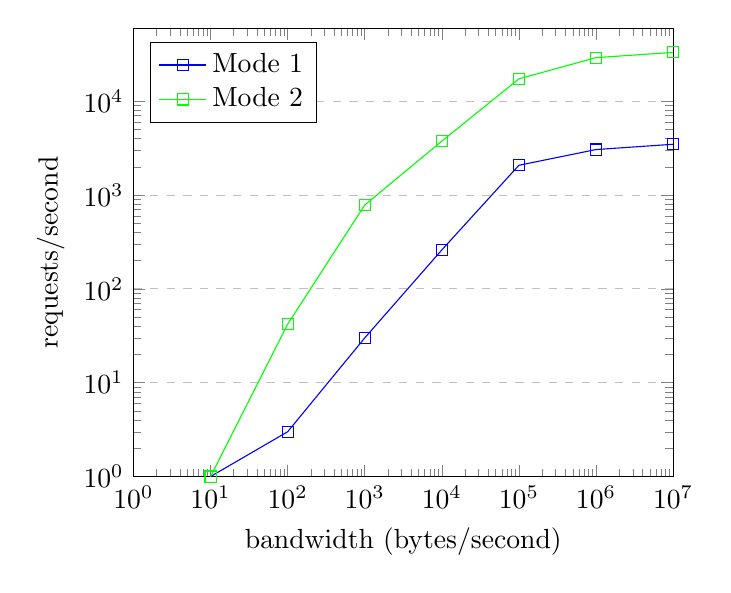
\begin{tikzpicture}
  \begin{loglogaxis}[
    %title={Bandwidth vs. Requests/Second},
    xlabel={bandwidth (bytes/second)},
    ylabel={requests/second},
    xmin=1, xmax=10000000,
    ymin=1, ymax=60000,
    xtick={1,10,100,1000,10000,100000,1000000,10000000},
    ytick={1,10,100,1000,10000},
    legend pos=north west,
    ymajorgrids=true,
    grid style=dashed,
    ]
    
    \addplot[
    color=blue,
    mark=square,
    ]
    coordinates {
      (10,1)(100,3)(1000,30)(10000,260)(100000,2077)(1000000,3056)(10000000,3478)
    };

    \addplot[
    color=green,
    mark=square,
    ]
    coordinates {
      (10,1)(100,42)(1000,783)(10000,3754)(100000,17317)(1000000,29143)(10000000,33169)
    };
    \legend{Mode 1,Mode 2}
    
  \end{loglogaxis}
\end{tikzpicture}
\caption{Bandwidth vs. performance}
\label{fig:band}
\end{figure}

\begin{figure}[t]
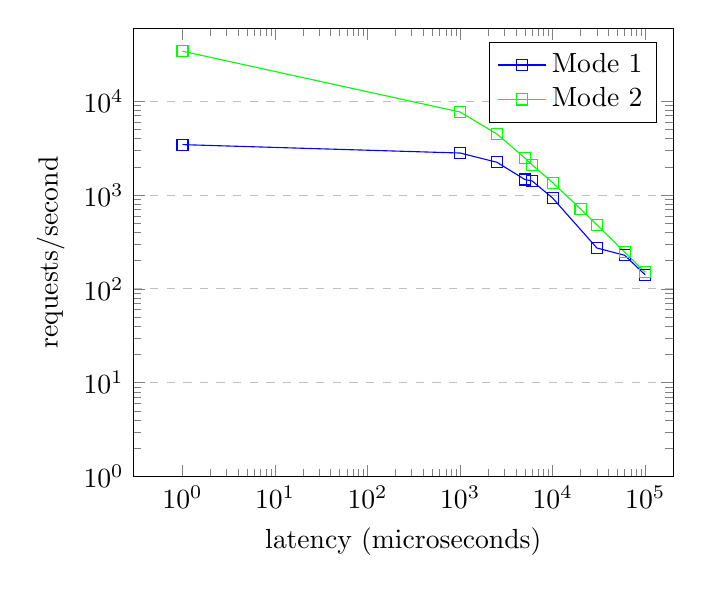
\begin{tikzpicture}
  \begin{loglogaxis}[
    %title={Latency vs. Requests/Second},
    xlabel={latency (microseconds)},
    ylabel={requests/second},
    xmin=-100, xmax=200000,
    ymin=1, ymax=60000,
    xtick={1,10,100,1000,10000,100000,1000000,10000000},
    ytick={1,10,100,1000,10000},
    legend pos=north east,
    ymajorgrids=true,
    grid style=dashed,
    ]
    
    \addplot[
    color=blue,
    mark=square,
    ]
    coordinates {
      (1,3448)(1000,2806)(2500,2235)(5000,1465)(6000,1413)(10000,928)(30000,273)(60000,228)(100000,141)
    };

    \addplot[
    color=green,
    mark=square,
    ]
    coordinates {
      (1,34121)(1000,7668)(2500,4470)(5000,2482)(6000,2089)(10000,1356)(20000,711)(30000,482)(60000,246)(100000,150)
    };
    \legend{Mode 1,Mode 2}
    
  \end{loglogaxis}
\end{tikzpicture}
\caption{Latency vs. performance}
\label{fig:late}
\end{figure}



To simulate different layouts of the three constituent parties, we ran our system as three types of processes on the same machine (running a AMD Athlon(tm) II P340 Dual-Core Processor), with artificial delays added between the resource device and the other two entities. Delays were added in two forms: as a raw latency value, and as a ``bandwidth'' value that increased the delay according to the size of the data transferred. A workload consisting of three clients, three resource processes, and one authority was created, with each resource process providing access to one resource (though support for multiple resources per resource process is complete). The performance was measured as the number of processed resource requests over the course of 5 seconds. As can be seen in Fig.~\ref{fig:band} and \ref{fig:late}, the results clearly show that Mode 2 is superior to Mode 1 in the majority of network conditions. While the results are not fine-grained enough to determine what specifically are the causes, there two intuitive reasons for this to be the case.

First, there is a considerable difference in the amount of cryptographic operations being done. In Mode 1, the integrity of the token received must be cryptographically verified each time a resource is accessed, as it contains the only available source of information to the resource device (aside from the public keys that are given out of band). In Mode 2, only when creating and destroying capabilities are cryptographic operations done (since accessing the resource is done via a random ``pointer,'' which functions as a password). Given that the creation and destruction of capabilities happens far less frequently than their being accessed, one source of these performance differences becomes clear.

The second major reason why Mode 2 would be so much faster than Mode 1 is that Mode 2 requires less data to be transferred over the wire. Again, because there are far fewer capabilities created than there are invocations of capabilities, that Mode 1 requires sending the entire capability along with metadata for every access means that much more traffic is being generated than Mode 2, which only needs to send the entire capability to the resource once. This comes at the cost of an extra round trip to the device when a resource is created. And as can be seen in Fig.~\ref{fig:late}, the cost of this extra round trip causes the advantage of Mode 2 over Mode 1 to become less and less, though never quite surpassing it (though it is almost certainly the case that a more creation-heavy workload would have seen Mode 1 outperform Mode 2).

In terms of memory usage, the maximum observed memory consumption of the device in Mode 1 was 5.9 MB, while the maximum observed memory of the device in Mode 2 was 2.2 MB. This difference is due to the extra overhead from storing additional cryptographic structures in Mode 1, and needing to store each capability as it is being processed for each request, even if the capability is the same as before. Again, in a workload that involves a larger number of capabilities (as compared to accesses) at one time, the results likely would have been much different.

These results, while still preliminary, are much more extensive than any of the results that were detailed in the paper presenting CapBAC.~\cite{hernandez2013distributed} In our results, we have shown that an alternative design, where security is based on the secrecy of a particular value (a ``pointer'') instead of full cryptographic verification for every request, could have provided much better performance.
